Recent studies on scaling laws~\citep{henighan2020scaling, hoffmann2022training, kaplan2020scaling} have underscored the predictable improvement in model performance with increases in computational budget, model size, and data size. Yet, identifying the most effective distribution of resources between model and data sizes upon expanding the computational budget remains a formidable challenge in the field of scaling laws. Additionally, research conducted by~\citet{deepseekai2024deepseek} has highlighted that the allocation of an increased computational budget towards model scaling should be proportional to the quality of the data available. In light of these insights, we propose a novel approach aimed at dynamically adjusting the resource allocation between data and model sizes through a series of staged training processes. This strategy iteratively fine-tunes the balance between data characteristics and model size according to scaling laws, enhancing both model training efficiency and performance.

\textbf{Method}\quad
Following the methodology outlined by~\citet{kim2023solar}, our goal is to upscale our Yi-6B base model, which has 32 layers, to a 9B model named the Yi-9B base model, featuring 48 layers, by duplicating the original 16 middle layers 12-28. Depth up-scaling involves expanding the base model's depth and subsequently continuing the pretraining phase for the enhanced model.

\begin{figure}[t]
  \centering
  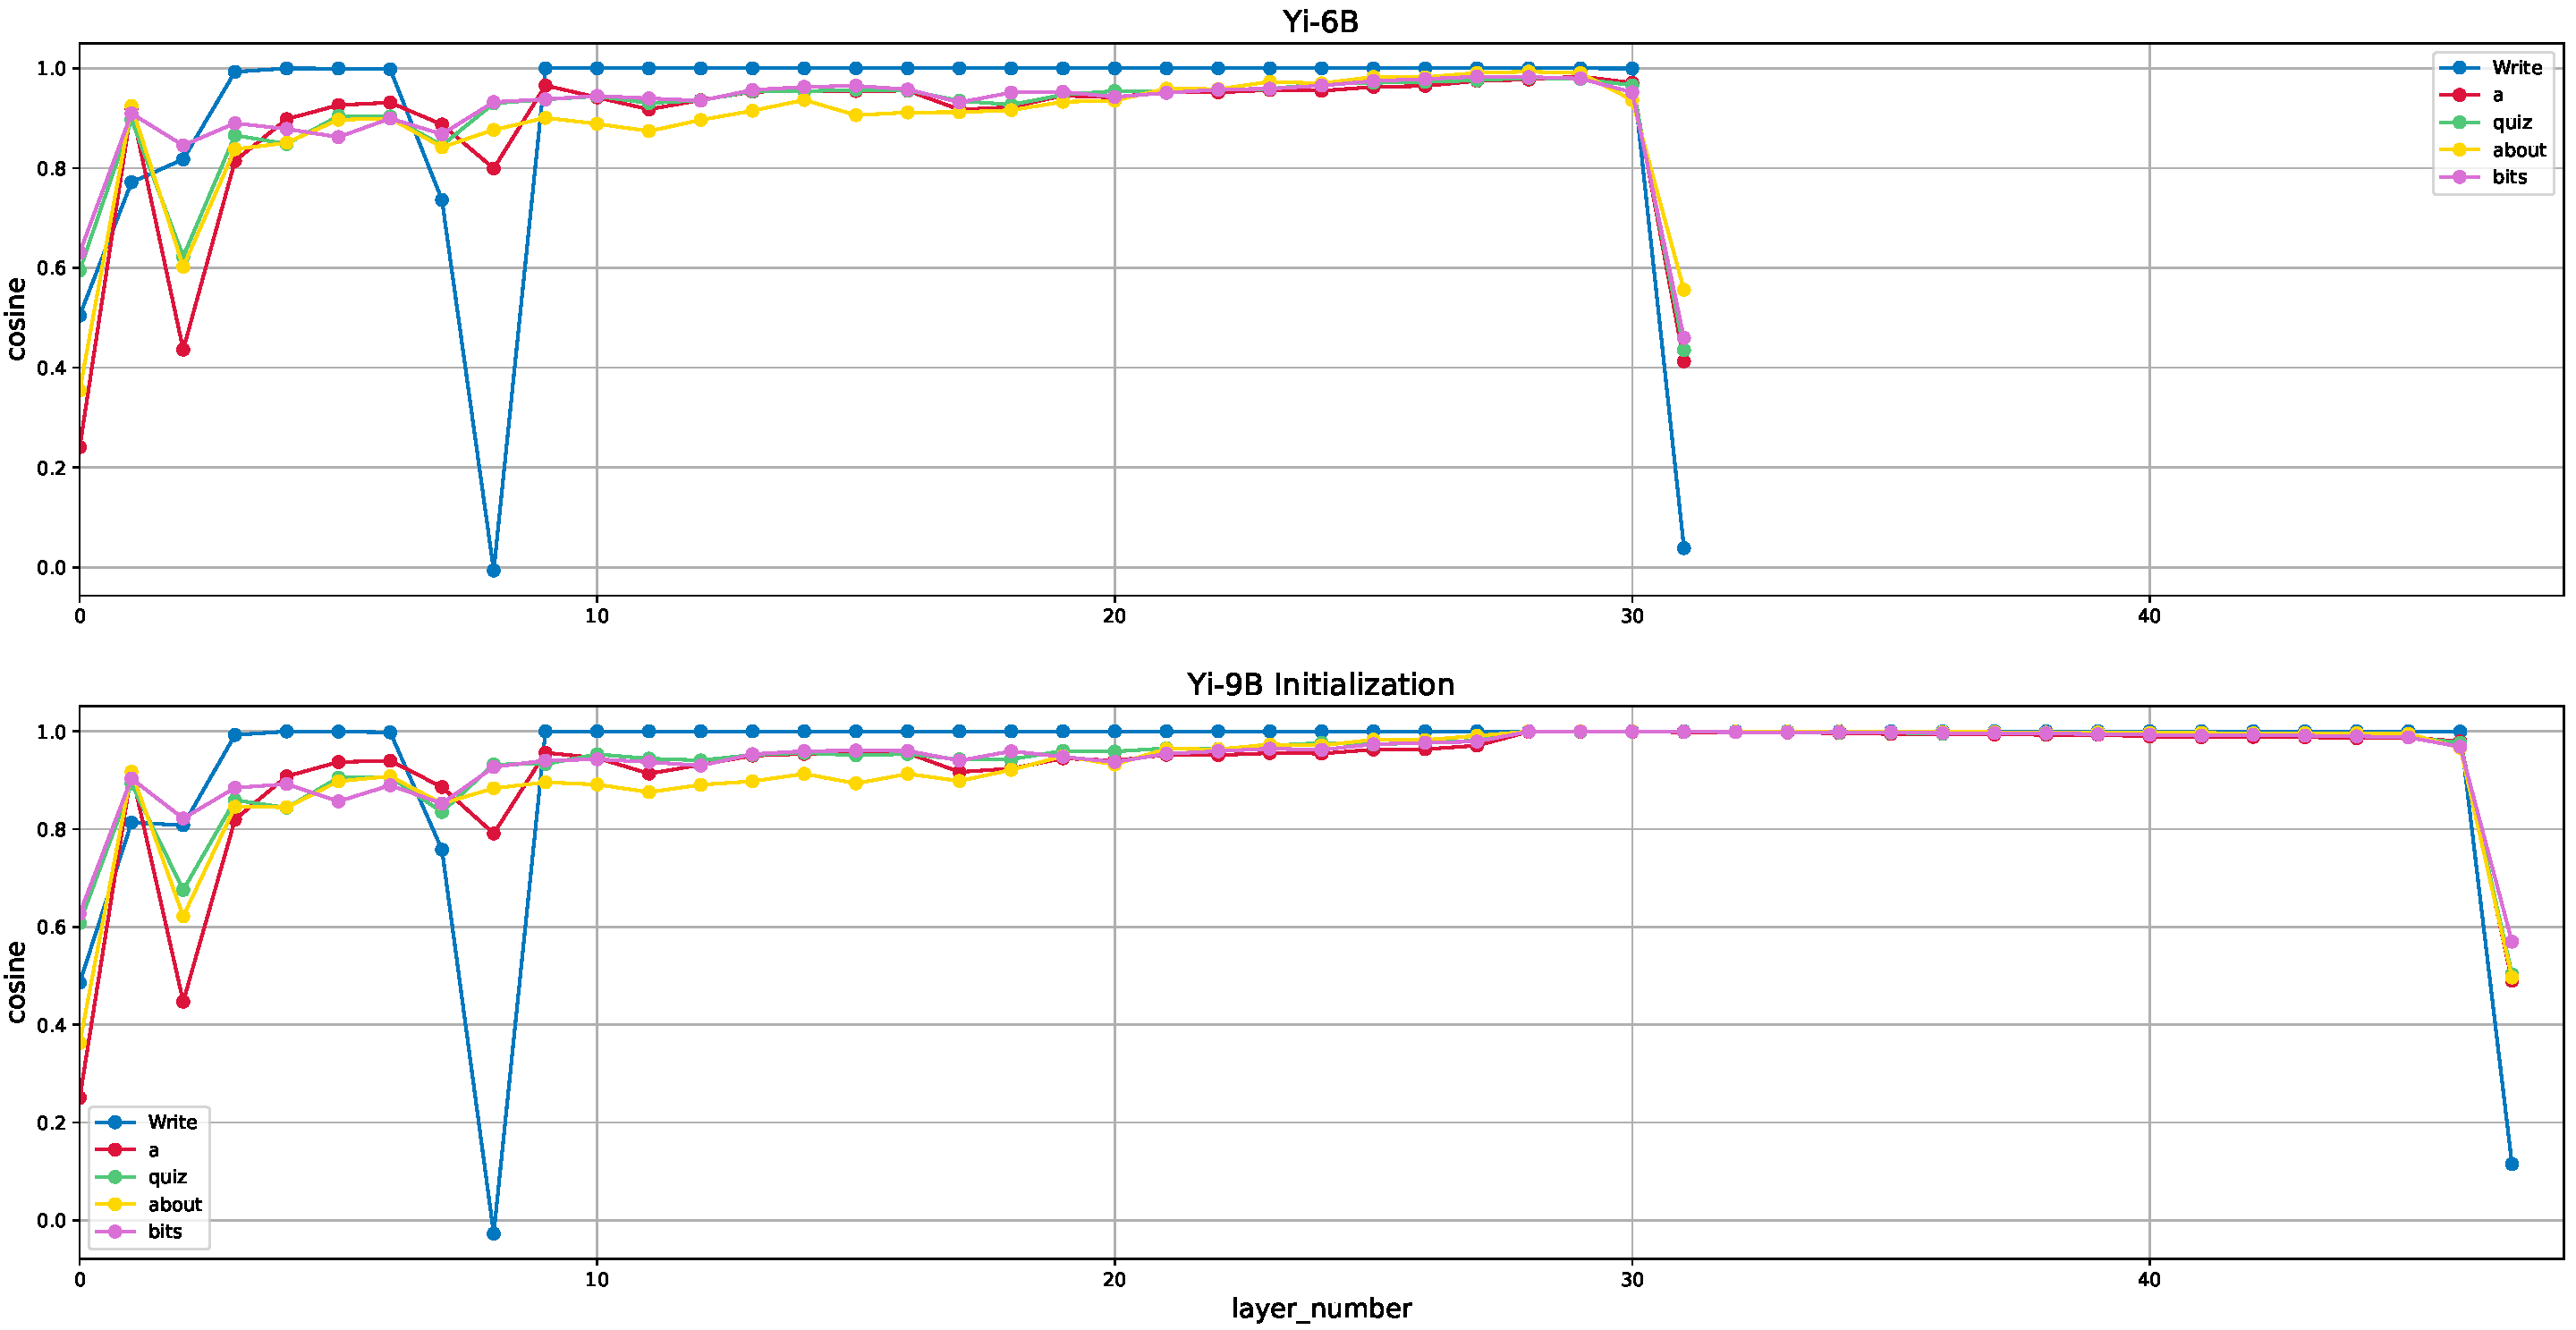
\includegraphics[width=0.9\textwidth]{images/layer_cosine_graph.pdf}
  \caption{Input/output cosine similarity score of each token per layer for text "Write a quiz about bits". The cosine similarity scores of the 16 newly added layers(layers 28-44), as depicted in the lower figure, are observed to be nearly 1.} 
  \label{fig:layer_cosine_score}
\end{figure}

Our investigations reveal that the decision on which layers to replicate could be informed by evaluating the cosine similarity scores between the inputs and outputs of each layer. Such an approach allows for targeted model scaling without necessitating additional pretraining, leading only to minimal performance impacts. This minimal impact on performance is attributed to the high cosine similarity, approaching one, between the inputs and outputs of the duplicated layers, as evidenced in Figure \ref{fig:layer_cosine_score}. This observation suggests that the replication of these layers does not significantly alter the output logits produced by the original model. This method ensures the efficient scaling of the model by optimizing its architecture based on the internal processing dynamics of its layers.

\begin{table*}[tb!]
\centering
\scalebox{0.8}{
\begin{tabular}{lcccccccc}
\toprule
\textbf{Model} & \textbf{Arc-C} & \textbf{HellaSwag} & \textbf{MMLU} & \textbf{Winogrande} & \textbf{GSM8K} & \textbf{MATH} & \textbf{HumanEval} & \textbf{MBPP} \\
\midrule
% \textbf{deepseek-6.7b}
% & 45.0 & 67.9 & 49.2 & 64.0 & 41.0 & 42.1 & 60.7 & 13.9 \\
% \textbf{Mistral-7B-v0.1}
% & 57.2 & 81.4 & 62.5 & 74.0 & 35.6 & 26.2 & 39.6 & 9.5 \\
% \textbf{solar\_10.7B}
% & 57.9 & 82.1 & 64.2 & 74.6 & 56.8 & 29.3 & 38.9 & 6.9 \\
\textbf{Yi-6B} & 50.3 & 74.4 & 63.2 & 71.3 & 32.5 & 4.6 & 15.9 & 26.3 \\
\textbf{Yi-9B Init} & 52.1 & 73.3 & 63.0 & 69.4 & 31.3 & 4.1 & 12.8 & 25.8  \\
\textbf{Yi-9B} & \textbf{55.6}  & \textbf{76.4} & \textbf{68.4} & \textbf{73.0} & \textbf{52.3} & \textbf{15.9} & \textbf{39.0} & \textbf{54.4} \\
\bottomrule
\end{tabular}
}
\caption{Performance between Yi-6B and Yi-9B: Arc Challenge (25-shot), HellaSwag (10-shot) MMLU (5-shot), Winogrande (5-shot), GSM8K (5-shot), MATH (4-shot), HumanEval pass@1, MBPP pass@1(3-shot). Yi-9B Init is just depthwise upscaling from Yi-6B by duplicating layers 12-28 without further training.}
\label{tab:depth_upscaling}
\end{table*}

\textbf{Continual Training}\quad
The dataset is composed of approximately 800 billion tokens across two stages, with around 70\% having been recently collected and carefully selected. We have enhanced the code coverage in the final stage to improve code performance.

To optimize the training process, we maintain a constant learning rate of 3e-5, and adopt a strategic approach to gradually increase the batch size from 4M tokens whenever the model's loss plateaued. This incremental adjustment of the batch size, alongside maintaining all other parameters in alignment with the established Yi-6B base model configuration, was instrumental in navigating the challenges of training at scale.

The effectiveness of these strategies is demonstrated in Table \ref{tab:depth_upscaling}, which details the Yi-9B base model's performance across a variety of benchmarks, including common sense, reasoning, knowledge, coding, and mathematics. It underscores the competitive advantages of Yi-9B base model in specific domains, illustrating the efficacy of our methodology in enhancing model performance by optimally adjusting the interplay between data characteristics and model size.


